%%%%%%%%%%%%%%%%%%%%%%%%%%%%%%%%%%%%%%%%%%%%%%%%%%%%%%%%%%%%%%%%%%%%%%%%%%%%
% Latex source file for the LCIO users manual
% the file can be processed with pdflatex and latex2html(using .jpg and .pdg) 
% and plain latex (using .eps) 
%
%  --- to create  an html file @ DESY (modify path accordingly for other sites) from this manual :
% /products/latex2html/latex2html-2002-1/bin/latex2html -mkdir -dir ../../../doc/manual_html -info 0 -no_auto_link -split 0 -no_navigation manual.tex 
% ----- or pdf:
% pdflatex manual.tex
% ----- or postscript:
% latex manual.tex ; dvips manual.dvi
%
%%%%%%%%%%%%%%%%%%%%%%%%%%%%%%%%%%%%%%%%%%%%%%%%%%%%%%%%%%%%%%%%%%%%%%%%%%%%
\documentclass[twoside]{article}
%\documentclass[twoside]{report}
% --- the following allows to use either latex/latex2html or pdf latex
% --- with the same file and have the right images included (eps or jpg/png)
\newif\ifpdf\ifx\pdfoutput\undefined\pdffalse\else\pdfoutput=1\pdftrue\fi
\newcommand{\pdfgraphics}{\ifpdf\DeclareGraphicsExtensions{.png,.jpg}\fi}
%-------------------------------------------------------------------------
\usepackage{graphicx}
%\usepackage{fancyhdr}
\usepackage{verbatim}
\usepackage{html}
%\pagestyle{fancy}
%\fancyhead{} % clear all fields
%\fancyhead[C]{\it {LCIO - Users manual}}
%\fancyhead[RO,LE]{\thepage}
%\fancyfoot{} % clear all fields
%\renewcommand{\headrulewidth}{0pt}
%\renewcommand{\footrulewidth}{0pt}
\renewcommand{\appendixname}{Appendix}

\newcommand{\captionstyle}[1]{\textit{\small{#1}}}

\newcommand{\Href}[1]{\htmladdnormallink{\footnotesize {#1}}{#1}}

\setlength{\textheight}{235mm}
\setlength{\textwidth}{155mm}
\setlength{\topmargin}{-20mm}
\setlength{\evensidemargin}{10mm}
\setlength{\oddsidemargin}{10mm}

%\setlength{\parskip}{\baselineskip}
\setlength{\parindent}{0pt}

\bibliographystyle{apsrev}

\begin{document}
\pdfgraphics

%\title{LCIO [v02-00] -  Users manual}
\title{{\Huge\bf LCIO  -  Users manual} \\ v02-00}

%\author{F. Gaede \\  DESY IT}
%\author{F. Gaede, H. Vogt \\  DESY IT, DESY Zeuthen}
\author{F. Gaede, DESY IT \\ H. Vogt, DESY Zeuthen}


\maketitle
\setcounter{tocdepth}{2}
\tableofcontents

%\thispagestyle{fancy}

\newpage
\section{INTRODUCTION \label{intro}}

{\bf Note: Some of the latest developments in LCIO are not yet described in this manual.
However it is still a good starting point if you are new to LCIO as it explains the basic concepts to quite 
some detail. For some of the newer developments and the current versions please refer to  the API documentation 
at} \Href{http://lcio.desy.de} {\bf and the discussions in the LCIO forum at } 
\Href{http://forum.linearcollider.org}.

LCIO is a persistency framework that defines a data model for the linear collider 
physics community. It is intended to be used in both simulation studies and 
analysis frameworks. Its light weight and portability makes it also suitable 
for use in detector R\&D applications. 

It provides a C++ and a Java implementation with a common interface (API).
A Fortran interface to the C++ implementation is provided as well.

This manual is intended for application developers that want to incorporate LCIO in their 
programs. This includes e.g. simulation developers as well as  physicists that want to 
read LCIO files for their analysis. It focuses on the practical aspects of using LCIO. A more 
general discussion can be found in \cite{lcio_chep} and other documents listed on the 
LCIO homepage~\cite{lcio_home}.

\section{Installation}
\subsection{Getting LCIO}
If LCIO is not yet installed at your site you can get a recent copy from the SVN repository as
follows {\it bash}:

\begin{verbatim}
  svn co svn://svn.freehep.org/lcio/tags/v01-60 lcio/v01-60 # checkout release v01-60
  svn co svn://svn.freehep.org/lcio/trunk lcio/trunk # checkout trunk
\end{verbatim}

\subsection{Requirements}
In order to build LCIO you need to have a Java VM (version 1.4 or higher) installed 
on your platform. This is true even if you only want to install the C++ version as the 
API-files are generated from an abstract description for Java and C++ using the 
AID~\cite{ref_aid} tool. The build scripts used in LCIO also require that \verb$gcc$ and 
\verb$gmake/make$ are installed.

The C++ version of LCIO is developed and tested under Linux (SL4 and SL5 32 and 64bit)
and also builds under Windows/Cygwin or MacOSX.

As the -ansi compiler flag is used it should be fairly easy to port it to other platforms with
an ANSI compliant C++ compiler.\\\\

\subsection{Building LCIO} \label{build_lcio}

There are two build tools that can be used to build LCIO: maven and CMake~\cite{ref_cmake}. 
CMake~\cite{ref_cmake} has been introduced in version v01-11 to facilitate cross plattform support for 
the C++ version. 

\subsubsection{Building LCIO with CMake}
If you want to use CMake for building LCIO you need at least CMake version 2.6.

%Some of the features CMake includes are:
%\begin{verbatim}
%  * Support for building shared libraries
%  * Generates native build files (e.g., makefiles on Unix; workspaces/projects on MS Visual C++)
%  * Support for out-of-source builds. Multiple build trees are possible from a single source tree.
%  * CMake is open source
%\end{verbatim}

If you want to build LCIO using CMake, make sure that the cmake command is in your path, e.g.\\

\verb|export PATH=Path_to_CMake/bin:$PATH|\\\\

Then issue the following commands:
\begin{verbatim}
  mkdir build           # <-- create an out-of-source directory for the build
  cd build
  cmake ..              # check build options ( change options with: cmake -DOPTION=ON|OFF .. )
                        #  e.g. to also build the Java version, use: cmake -DINSTALL_JAR=ON ..
                        #  optionally use: ccmake .. and configure interactively
  make install
\end{verbatim}

CMake options may also be specified in a separate file and read with the -C option. (please check the CMake~\cite{ref_cmake} documentation for more details)
\begin{verbatim}
  # ILCSoft.cmake is a configuration file generated for each ilcsoft reference installation. It contains the list of paths from all tools within the installation.
  # in this example the BUILD_ROOTDICT option from LCIO is activated which requires the path to the ROOT package. This path is read from the ILCSoft.cmake configuration file.
  cmake -C /afs/desy.de/project/ilcsoft/sw/i386_gcc41_sl5/v01-11/ILCSoft.cmake -DBUILD_ROOTDICT=ON ..
\end{verbatim}

\subsubsection{Building LCIO with ant}

% TODO need to update this section for using maven

A few variables have to be set depending on your development environment, e.g.
\begin{itemize}
\item{ {\bf Linux (and bash):} 
\begin{verbatim} 
  export LCIO=/lcio/v02-00                <-- modify as appropriate
  export PATH=$LCIO/tools:$LCIO/bin:$PATH

  export JDK_HOME=/usr/lib/j2sdk             <-- modify as appropriate

  ( export CLHEP=/opt/products/CLHEP/2.0.4.5  <-- optionally use CLHEP four vectors with LCIO/C++) 
\end{verbatim} 
}
%$ <- fixes syntax highlighting
\item{ {\bf Windows/Cygwin - DOS shell:} 
\begin{verbatim}
  set PATH=c:/cygwin/bin;%PATH%            <-- modify as appropriate

  set LCIO=c:/lcio/trunk                   <-- modify as appropriate
  set JDK_HOME=c:/j2sdk1.4.1_01            <-- modify as appropriate 

  set PATH=%LCIO%/tools;%LCIO%/bin;%PATH%
\end{verbatim}
Note: Cygwin is only needed for gcc and make to build the C++ version.
}
\item{ {\bf Windows/Cygwin - Cygwin shell (bash):} 
\begin{verbatim}
  export LCIO=/cygdrive/c/lcio/trunk             <-- modify as appropriate
  export PATH=$LCIO/tools:$LCIO/bin:$PATH
  export JDK_HOME=/cygdrive/c/j2sdk1.4.1_01      <-- modify as appropriate
\end{verbatim} %$
}
\end{itemize}


To build the Java and C++ versions use the following commands\footnote{When using the Cygwin shell you need to
call the Windows version of ant with its full name, i.e. {\em ant.bat cpp}.}:
\begin{verbatim}
  ant aid.generate     <-- generates common API
  ant cpp              <-- creates C++ version
  ant aid              <-- creates Java version
  ant f77              <-- builds f77 examples
\end{verbatim}
or all in one:
\begin{verbatim}
  ant aid cpp f77
\end{verbatim}
or if starting over from a previously failed attempt to build LCIO:
\begin{verbatim}
  ant clean aid cpp f77
\end{verbatim}



Both ways of building LCIO will create the following libraries and executables:

\begin{verbatim}
 ./lib
      lcio.jar       <-- Java library (and executables)
      liblcio.so     <-- C++ lcio library
      libsio.so      <-- C++ sio library

 ./bin               <-- C++ examples and tools
      anajob
      copyfix
      dumpevent
      readcalibration
      recjob
      simjob
      lcio_event_counter
      stdhepjob

 ./bin               <-- f77 examples
      anajob_F
      simjob_F
      recjob_F 

\end{verbatim}


\subsection {Checking the Installation}

To check whether the (C++) installation was successful run the {\it simjob} program:
\begin{verbatim}
  simjob simjob.slcio
\end{verbatim}
This creates a simple LCIO file that you can read with 
\begin{verbatim}
  anajob simjob.slcio
\end{verbatim}
The same for the Java - Linux version:
\begin{verbatim}
  runSimJob.sh simjob.sclio
  runAnalysisJob.sh simjob.sclio
\end{verbatim}
or for the Java Windows (Cygwin) version:
\begin{verbatim}
  runSimJob[.bat] simjob.sclio
  runAnalysisJob[.bat] simjob.slcio
\end{verbatim}
In case CMake has been used to build LCIO it is possible to run a small chain of tests by calling:
\begin{verbatim}
  make tests && make test
\end{verbatim}



\subsection {Building the documentation} \label{build_doc}

A few targets are defined to build the documentation (see below), that is also available
from the LCIO homepage~\cite{lcio_home}, see (\ref{sec_api}).\\

If you are using CMake (see \ref{build_lcio}) all documentation can be built and installed
by setting the cmake option  \verb|INSTALL_DOC| to ON as follows:
\begin{verbatim}
  cmake -DINSTALL_DOC=ON ..
  make install
\end{verbatim}

In order to build individual documentation components the following targets may be used:
\begin{verbatim}
  make doc              <-- build all documentation (doc_cpp + doc_java + doc_manual)
  make doc_cpp          <-- C++ API documentation (needs {\em doxygen}~\cite{ref_doxygen})
  make doc_java         <-- Java API documentation
  make doc_refman       <-- Reference manual
  make doc_usrman       <-- User manual
\end{verbatim}

If you are not using CMake keep on reading the rest of this section on how to build
the documentation with ant:\\

You can create the documentation of the Java API with {\em javadoc}~\cite{ref_javadoc}:
\begin{verbatim}
  ant doc 
\end{verbatim}
and then open the file \verb|${LCIO}/doc/api/index.html| with your Browser. %$

\vspace{\baselineskip}
And the current version of this manual is created with
\begin{verbatim}
  ant doc.manual
\end{verbatim}
as \verb|${LCIO}/doc/manual.pdf| and \verb|${LCIO}/doc/manual.ps| provided you have latex in your 
\verb|$PATH| %$

%\newpage
\section{Using LCIO}
This section gives an introduction on how to use LCIO. We describe the user interface, the data model and
provide some code examples. For most of the section we focus on Java and C++ as these are the main 
languages supported by LCIO. Thanks to the AID~\cite{ref_aid} tool Java and C++ hava an API which is generated
from a common source and thus very similar.
The Fortran interface, implemented as a wrapper to the C++ implementation, is described 
in \ref{f77api}. 

\subsection{Java and C++ API} \label{sec_api}
Detailed documentation of the API is provided both for Java and C++ on the 
LCIO homepage~\cite{lcio_home} generated directly  from documentation in the source code using 
{\em javadoc} and {\em doxygen} respectively.   
If you are experienced in either Java or C++ you will probably  find most of what you need to use LCIO in the 
corresponding version of the API documentation. However, reading the detailed description of the data entities in 
[\ref{sec_datamodel}] is probably usefull.
 
A few words on the design of LCIO might be helpful\ to browse the documentation.
LCIO is organized in a hierarchical package structure where the packages combine classes
with a well defined purpose as shown in table~\ref{tab_pkg}.  
\begin{table}[h]
\begin{center}
\begin{tabular}{|c|c|p{6cm}|}
\hline
\rule[-5mm]{0mm}{10mm} C++ Namespace  &  Java package    &  Purpose \\ \hline \hline

 EVENT  &  hep.lcio.event   & The base interfaces of all data classes in LCIO. To be used for reading existing
 data.\\ \hline
 IO  &  hep.lcio.io   &  The base interfaces for io of data.\\ \hline
 IMPL  &  hep.lcio.implementation.event   & The (default) implementations of
 the base interfaces that are defined in EVENT. Needed for writing new data or extending existing data, e.g.
 during reconstruction. \\ \hline
 UTIL  &  hep.lcio.util   & Holds convenient and support classes and methods for the LCIO objects.
 \\ \hline
lcio  &   n.a. & The namespace lcio combines EVENT, IO, UTIL and IMPL for user convenience
(\#include "lcio.h"). \\ \hline
   \multicolumn{3}{|c|}{\textit{\small Namespaces/packages below are shown for completeness only, don't use 
 in your code!}}         \\ \hline
 IOIMPL  &  hep.lcio.implementation.io   &  Extensions to the default implementations
 needed for IO. With the exception of LCFactory all other classes are for internal use only.\\ \hline
 SIO  &  hep.lcio.implementation.sio   & The persistency implementation using SIO.
 Users should not use any of the classes defined here explicitly but through their
 base interfaces defined in IO. \\ \hline
 \textit{\small (DATA)  } &   \textit{\small (hep.lcio.data)}   & Removed in v1.3  \\ \hline

\end{tabular}
\end{center}
\caption{\captionstyle{ Overview of the packages (namespaces) used in LCIO.}}
\label{tab_pkg}
\end{table}
So a good starting point to browse the API documentation is the package/namespace overview.
Depending on the use case you will need mostly classes from one or two namespaces, e.g. if you need 
to read data from an existing LCIO file, you only need the classes in EVENT.
If you want to write data with LCIO you have to instantiate the implementation classes provided in 
IMPL (or implement the interface from EVENT).

%\begin{figure}
%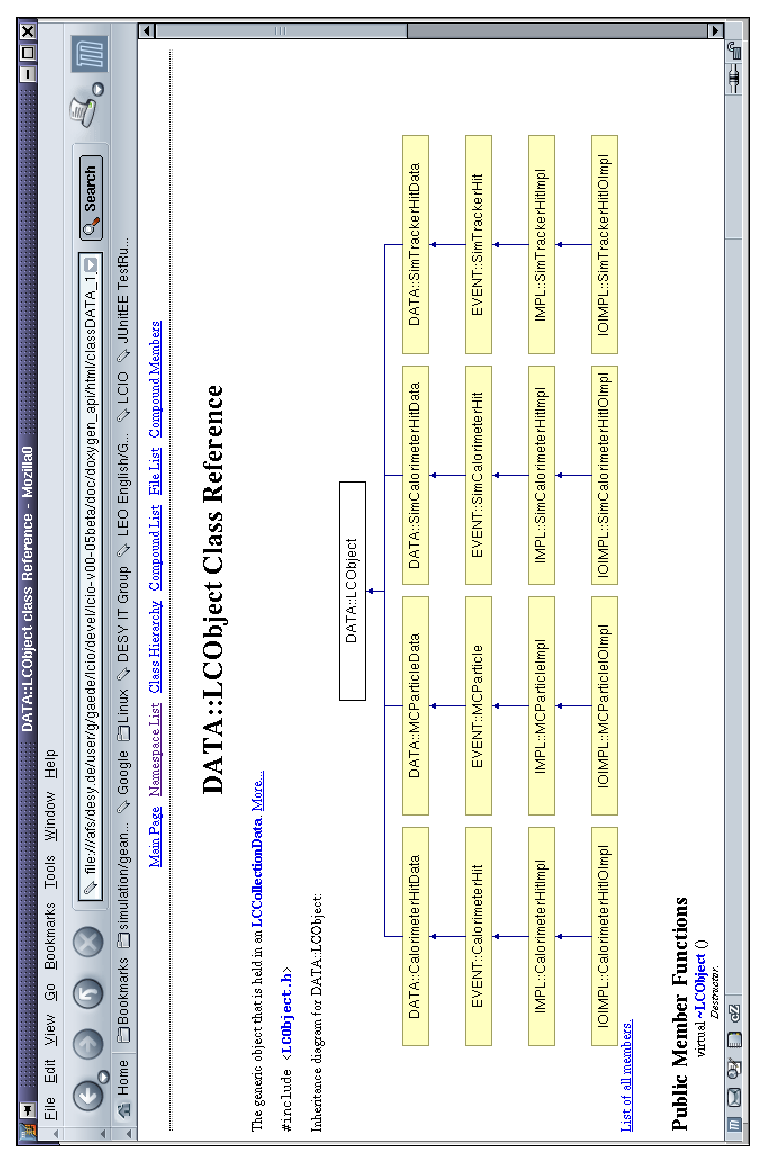
\includegraphics[width=145mm]{cpp_api}   
%\caption{Documentation of the C++ API. The class description of {\em LCObject} gives you fast access 
%to all data entities (classes). This class hierarchy also reflects the package hierarchy of LCIO.
%\label{fig_cpp_api} 
%\htmladdnormallink{(click here for a better quality image)}{../cpp_api.jpg}
%}
%\end{figure}


\subsubsection{Exceptions} \label{exceptions}
Both the Java and C++ versions of LCIO make use of the exception mechanism. Exceptions are 
implemented differently in Java and C++\footnote{The Java Exception mechanism is more powerful 
in that it offers compile time check of correct {\em try-catch} blocks or {\em throw} clauses 
and the notion of {\em unchecked} and {\em checked} exceptions.}. 
For LCIO we adopted a scheme of using exceptions that 
hides these differences as much as possible. All Exceptions except \verb$IOException$ in Java inherit 
from \verb$RunTimeException$, i.e. are {\em unchecked} exceptions. Thus the compiler will in general 
not complain about missing catch blocks or throw declarations. The same holds true for the C++ compiler 
anyhow.

In the API you will find {\em throw} clauses/declarations at certain methods. These are meant as a hint
to the user of what could go wrong in the method at hand - do not try to catch all exceptions with a 
dedicated {\em try-catch} block around every function call. Most exceptions will be due to 
{\em programming errors} and will cause an abort of the program -- when not caught by the user -- 
which is usually what you want.\\
There are exceptions to this rule however. In particular the \verb$DataNotAvailableException$ will be
thrown by methods accessing event data that are not available, e.g. if you are trying to get a named 
collection from the event that is not available. 
In this case it depends on your application whether you want to continue or not - if the 
computation is vital for the rest of the program you'll probably want to abort - if the code just
produces some check plots for a particular subdetector you might as well carry on with other 
7modules.\\
In case an exception is thrown at run time that is not caught the program will abort and you will get 
some printout as to what caused the exception - 
in Java this is done by the VM in C++ we print the type of the exception with some information on the 
problem (usually the class and function name).

\vspace{\baselineskip}
{\it {\bf Note to C++ programmers:} We included \verb$std::exception$ in all {\em throw} clauses in 
C++. This way we ensure a behavior similar to Java, i.e. despite a {\em throw}
clause basically all exceptions can be thrown by the function, as all STL-Exceptions 
as well as all LCIO-Exceptions inherit from the base \verb$std::exception$. So the user can decide to
catch {\em run time} exceptions for parts of the code in order to prevent an abort of the program. 
}

\subsection{Data model \label{sec_datamodel}}

Figure~\ref{fig_eventdata} shows the event data model of LCIO. The most important class is LCEvent, it serves as a 
container for all data that are related to one event. It holds an arbitrary number of named collections 
(class LCCollection) of data objects (class LCObject). 
Run related information is stored in LCRunHeader. Run-headers, events and collections have an instance of 
LCParameters that allows to attach arbitrary named parameters of types  \textit{int, float} or \textit{string}
to either of these objects. This mechanism is foreseen to allow storage of meta data, e.g. the name of the 
algorithm that has been used to create a certain collection.
The LCCollection has a type word that is used as a flag word, where certain bits are used by LCIO to denote some
well defined feature of the objects in the collection. Typically these flag bit positions are defined as global
constants in the class LCIO.


\begin{figure}
%\htmlimage{flip=r270}
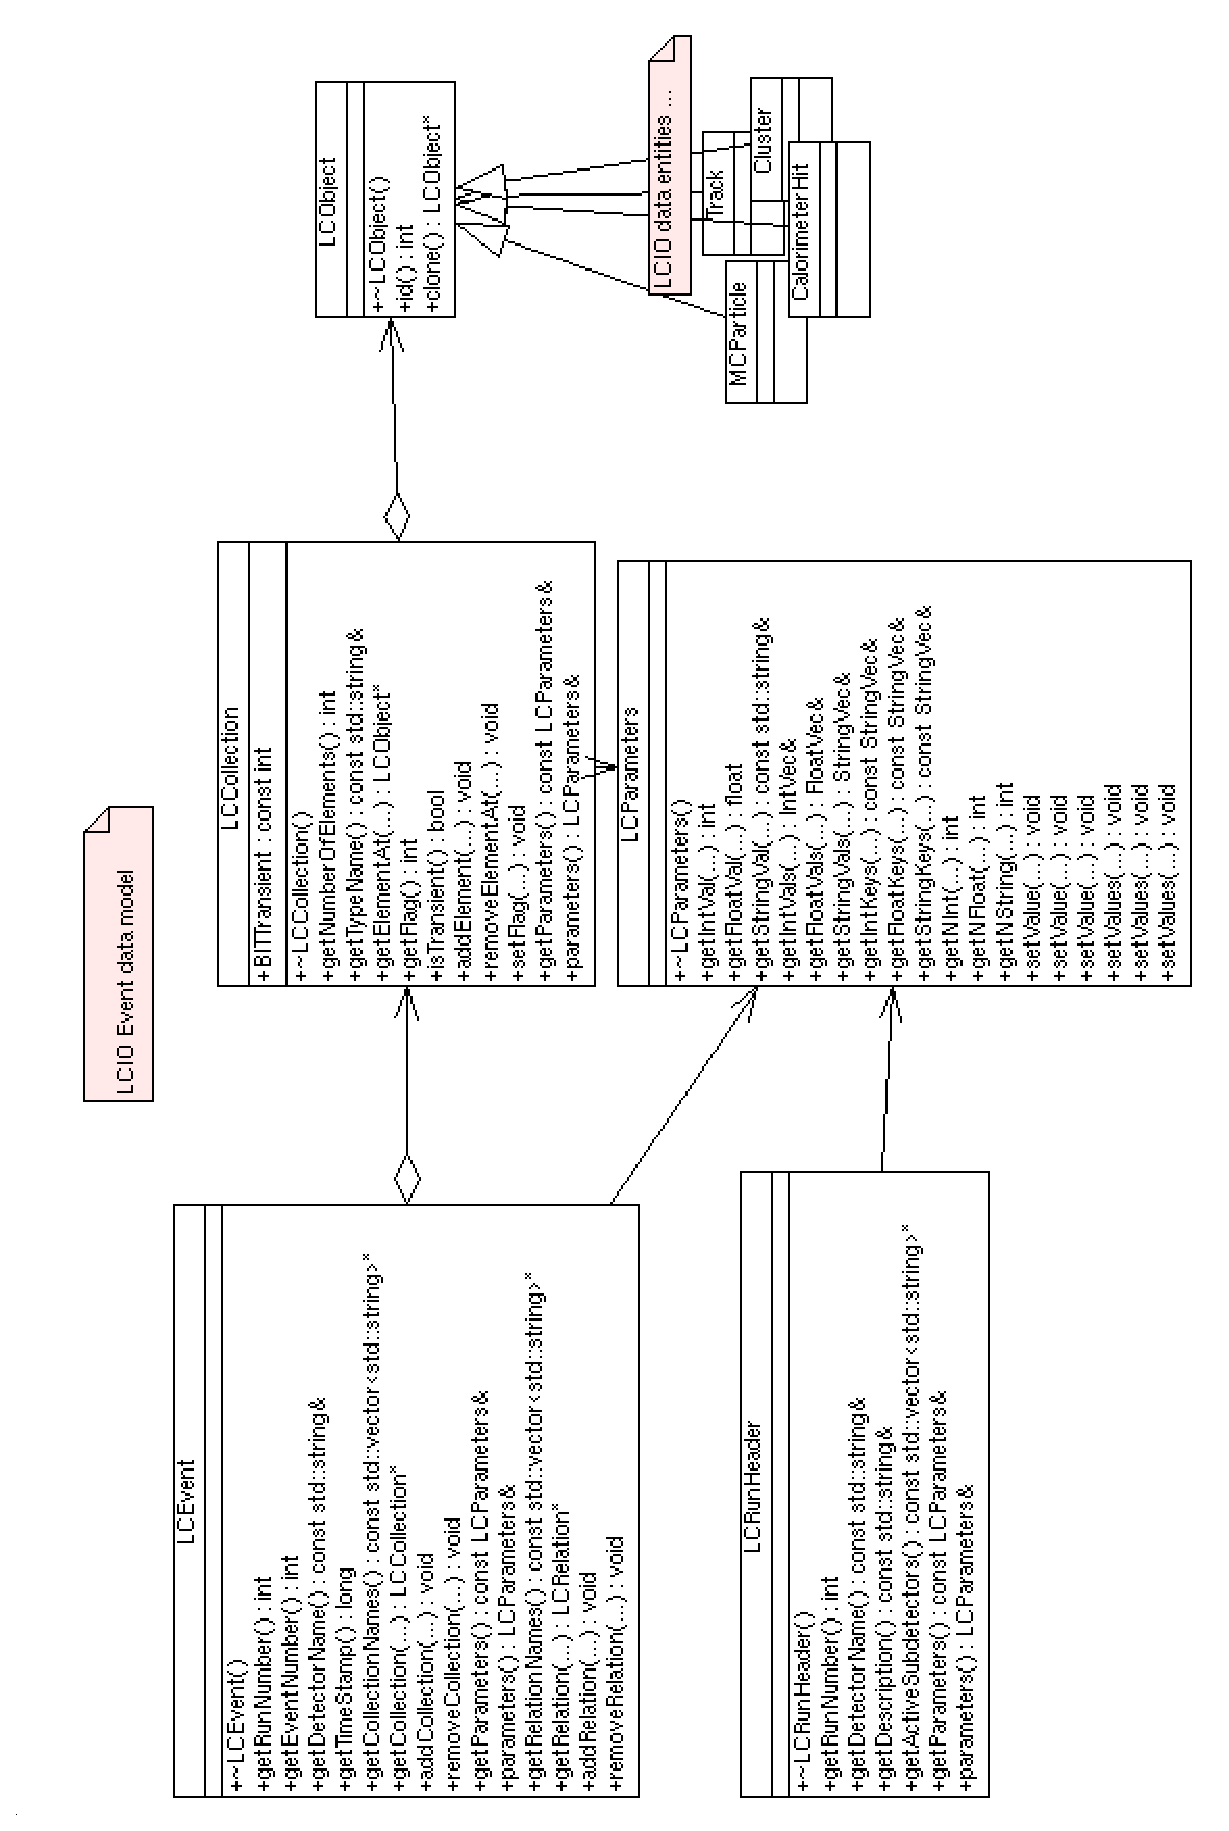
\includegraphics[width=150mm]{eventdata}    
\caption{\captionstyle{Overview of the event data model defined by LCIO.
The boxes correspond to classes and the arrows denote relationships between these. The main class in LCIO 
is LCEvent that serves as a container of named collections (LCCollection) of data objects (LCObject).
All data that are related to one event is stored in such collections (A few example classes are shown, see 
\ref{fig_lcobjects} for details on the data entities.) The LCRunHeader is used to store run related 
information. The class LCParameters can be used to attach keyed parameters of type \textit{int, float, string}
to either LCRunHeader, LCEvent or LCCollection in order to store so called meta data, e.g. the encoding of certain 
bits in some type word, or the order of some parameters in a given array.\label{fig_eventdata}
}}
\end{figure}

The following gives a detailed description of the data entities that are defined in LCIO. An overview of 
these classes is shown in figure~\ref{fig_lcobjects}.

\begin{figure}
%\htmlimage{flip=r270}
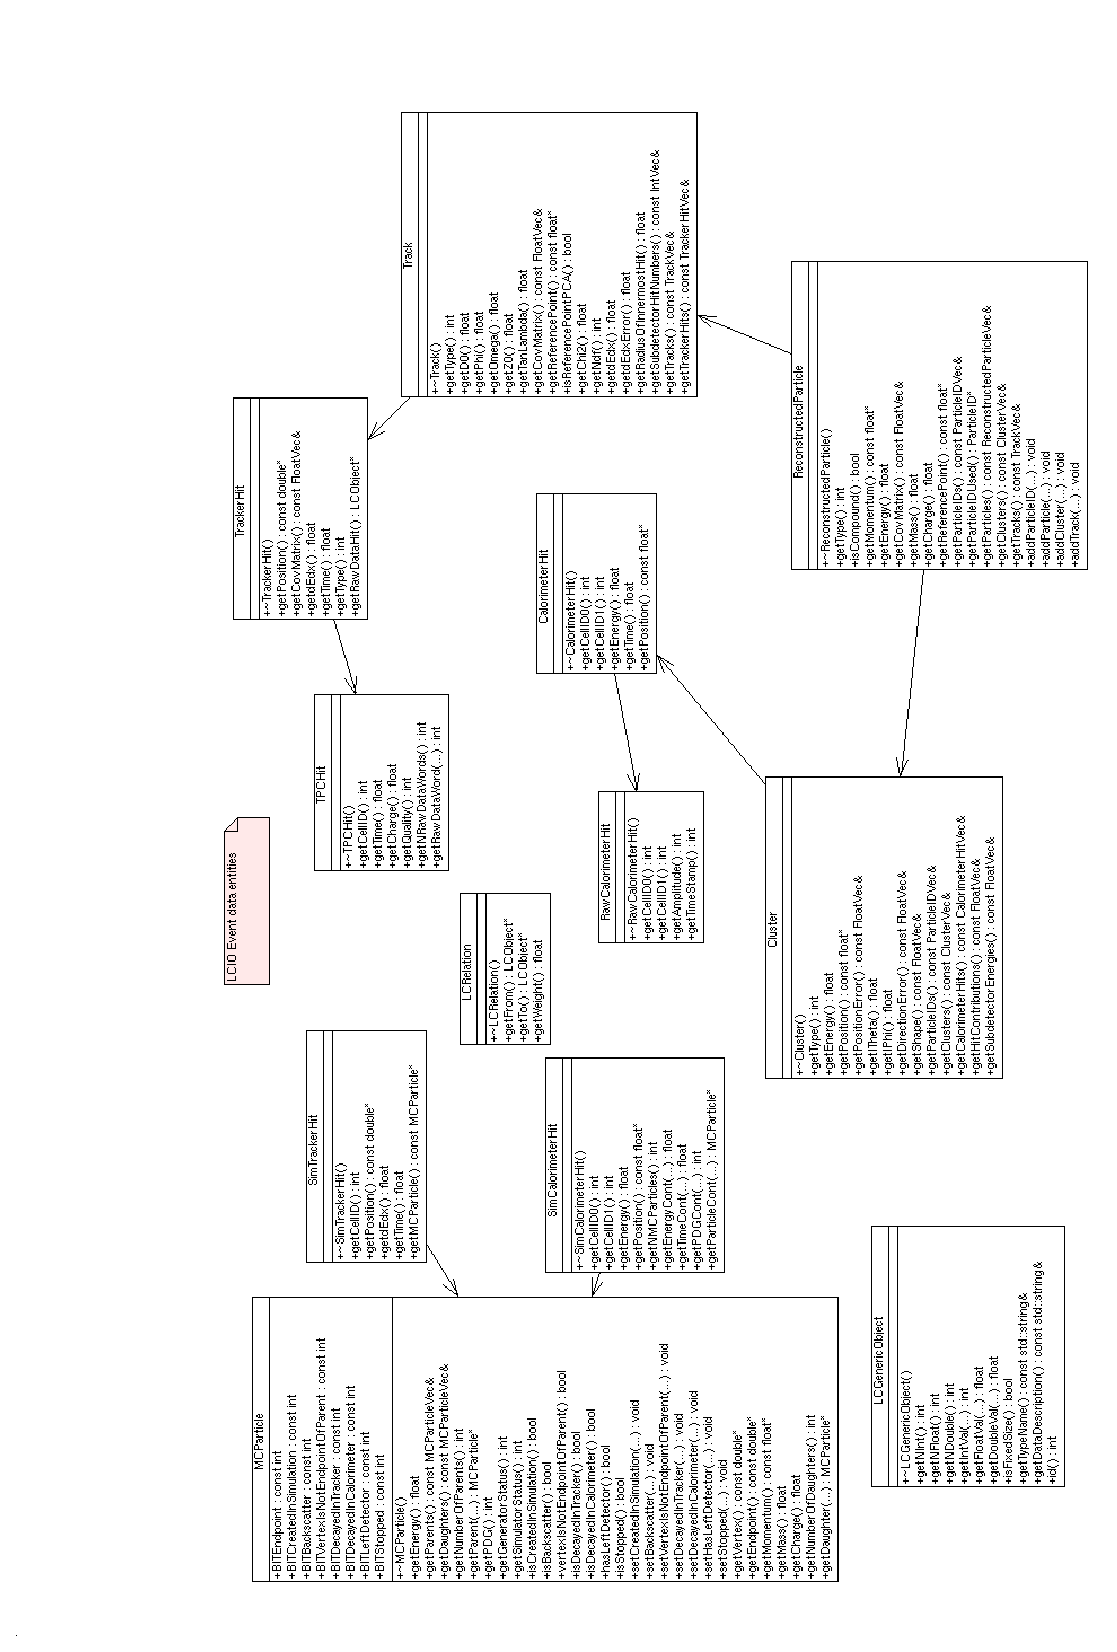
\includegraphics[width=150mm]{lcobjects}    
\caption{\captionstyle{Overview of the data entities defined by LCIO (namespace EVENT). 
All classes are subclasses of LCObject. The shown dependencies correspond to links between objects, e.g.
for a given reconstructed particle you can get the tracks and clusters that have been used to create the particle.
There is no direct link from 'real data' objects to Monte-Carlo objects, instead LCRelation is to be used for 
that.\label{fig_lcobjects}
}}
\end{figure}

\subsubsection{MCParticle}
There will be exactly one collection with name ``MCParticle'' in every event that holds 
the Monte Carlo truth particles as generated by the generator or as added by the simulation program
(decay in flight). Particles that are created during simulation will be added to the existing list of MCParticles.
Adding particles with their correct lineage ceases when a particle decays or interacts in a non-tracking region.
(Otherwise the number of MCParticles explodes in calorimeter shower development).
All energy depositions are assigned to the initial particle that decayed or interacted in a non-tracking region.
The exception is a particle producing a hit in a tracker. This particle is recorded, with the tracker hit 
assigned to it, and the particle is flagged as a "backscatter". Thus direct tracker hits for a particular 
particle can be distinguished from those not actually produced by that particle. 

The {\em generatorStatus} and {\em simulatorStatus} attributes define the creation and destruction
status of the particle, where the  {\em generatorStatus} is defined by the generator program and
the  {\em simulatorStatus} is combined from the following boolean flags:
\begin{itemize}
\item{{\bf isCreatedInSimulation} \\
True if Simulator created particle. False if Generator created particle.}
\item{{\bf isBackscatter} \\
True if particle created by Simulator as a result of interaction or decay in non-tracking region.
By convention, such particles are not saved. However, if this particle creates a tracker hit, the particle 
is added to the MCParticle list with this flag set,  and the parent set to the particle that initially decayed or
interacted in a non-tracking region}
\item{{\bf vertexIsNotEndpointOfParent} \\
True if particle created as a result of a continuous process where the parent particle continues, i.e. 
hard ionization, Bremsstrahlung, elastic interactions, etc.}
\item{{\bf isDecayedInTracker} \\
True if the particle decayed or interacted (non-continuous interaction, particle terminated) in a tracking region.}
\item{{\bf isDecayedInCalorimeter} \\
True if tracking of particle stopped because particle left the world volume.}
\item{{\bf hasLeftDetector} \\
True if tracking of particle left the world volume.}
\item{{\bf isStopped} \\
True if particle lost all kinetic energy inside world volume and did not decay.}
\end{itemize}

For the {\em MCParticle} only parent relationships are stored. When reading the data back from the 
file the daughter relationships are reconstructed from the parents. This is to ensure consistency.
Care has to be taken when analyzing the particle 'tree'. Because a particle can have more than one 
parent the particle list in fact does not consist of a set of trees (one for each mother particle) 
but  forms a 'directed acyclic graph'. Thus the user has to avoid double counting in his code.
Of course this only matters at the parton level, as real particles have exactly one or no parent. \\


\subsubsection{SimCalorimeterHit}
Generic class for calorimeter hits from a simulation program. Typically every calorimeter subdetector
will create a collection of this type. SimCalorimeterHits have a float energy amplitude and an int cellid,
and optionally a 3d hit/cell position. 
In order to study clustering and reconstruction algorithms there are links to the MCParticles that contributed 
to the hit. There are two different levels of detail foreseen( check/set the flag LCIO.CHBIT\_STEP):
\begin{itemize}
\item{LCIO.CHBIT\_STEP=0, normal mode: one MCParticle contribution for every MCParticle that contributed to the 
hit, i.e. there will be only one MCParticle contribution except for cells where showers from two particles 
overlap.}
\item{LCIO.CHBIT\_STEP=1, detailed mode: one contribution for every simulator step that contributed to the hit.
Every contribution has the energy, time and PDG of the shower particle that caused  the energy deposit.
This mode will result in a lot of entries per calorimeter hit and is intended for detailed studies only. }
\end{itemize}
In general the position of calorimeter hits will be decoded from the cellid to save disk space. For user 
convenience it is however possible to store the three dimensional position of the cell with every hit.
Check/set the collection flag bit LCIO.CHBIT\_LONG=1.
Also for cases where it is impossible or inconvenient to decode the cellid in one word, SimCalorimeterHit can have 
an optional second cellid (LCIO.CHBIT\_ID1=1). 

\subsubsection{SimTrackerHit}
This is the generic class for storing simulated hits from tracking subdetectors. It records the spacepoint,  
energy and time of the hit as well as a link to the MCParticle that caused it.

\subsubsection{RawCalorimeterHit}
This class is intended to be used for real calorimeter data, e.g. from test beam calorimeters.
It stores a cellid, amplitude and optionally (LCIO.RCHBIT\_TIME=1) a time word, all as int values as 
this is what is read out from the DAQ system. Also a second cellid can be utilized if needed (LCIO.RCHBIT\_ID1=1).
To save disk space when storing raw data only, set the colelction flag bit LCIO.RCHBIT\_NO\_PTR=1, 
suppressing an additional 32-bit  pointer tag per hit.

\subsubsection{CalorimeterHit}
The CalorimeterHit should be used for final reference to the calorimeter hits, i.e. after calibration, 
clustering etc. It has a float energy and optional time word. Clusters will have links to objects of type 
CalorimeterHit.

\subsubsection{TPCHit}
Deprecated. Please use the new classes for raw tracker data: TrackerRawData, TrackerData and TrackerPulse.
%As the name suggests this class has been specifically designed for TPC-like subdetector's raw data.
%It has a cellid, time and charge of the hit after feature extraction. Optionally (LCIO.TPCBIT\_RAW=1) raw
%waveforms can be stored in the hit as well. As for RawCalorimeterHit in a pure raw data stream a 32-bit pointer tag
%per hit can be suppressed (LCIO.TPCBIT\_NO\_PTR=1).

\subsection{TrackerRawData}
Generic class for raw tracker data. One or optionally two (LCIO.TRAWBIT\_ID1=1) cell ids can be used to decode the
readout channel. Specific subdetectors will use different encodings, e.g. a silicon vertex detector might use 
cellID0 and cellID1 to encode the module number, row and column of the hit. An arbitrary number of ADC values can be 
stored in the hit. This can be either a complete spectrum (waveform) as for a TPC like detector or just one or two 
consecutive ADC readout values.

\subsection{TrackerData}
Same as the TrackerRawData, except that the data has been corrected (calibrated). In particular the calibrated ADC 
values are stored as floating point charge values with arbitrary, i.e. subdetector specific units. 

\subsection{TrackerPulse}
Tracker pulse that is typically created from TrackerData by some sort of feature extraction, e.g. for a TPC like detector
the pulse will contain the integrated charge of the spectrum and the corresponding time.


\subsubsection{TrackerHit}
The TrackerHit serves as a generic hit type that can be used for pattern recognition. It allready has a space 
point position and error matrix, computed from the raw data. TrackerHits point back to the raw data hits that they
have been created from.

\subsubsection{Cluster}
Clusters are made from sets of CalorimeterHits that they point back to. Clusters can also be combined from other
Clusters allowing a tree-like structure, e.g. one could build clusters with a geometrical algorithm and then
combine some of these clusters to 'particles' applying some track-match criterieon. Due to the imaging capabilities
of the LC calorimeters, clusters have an intrinsic direction, denoted ITheta, IPhi. For fast Monte Carlo or in case
where the hits are droped from the files (DST) Clusters can have vector of subdetector energies. Check/set the 
collection variable ClusterSubdetectorNames for the decoding of the indices in the vector.
And similarly check/set the collection variable ClusterShapeParameters for the indices in the shape parameter 
vector. Clusters have a type word where the lower 15 bits can be used to decode the type of the cluster by the
user, e.g. define a bit per subdetector. Check/Set the collection variables ClusterTypeBitNames and 
ClusterTypeBitIndices.



\subsubsection{Track}
For LCIO we use the following parameters for Track:
\begin{itemize}
\item{{\bf d0}\\
Impact paramter of the track in the r-phi plane.}
\item{{\bf phi}\\
Phi of the track at the reference point.}
\item{{\bf omega}\\
The signed curvature of the track in [1/mm] - the sign is that of the particle's charge.
}
\item{{\bf z0}\\
Impact paramter of the track the in the r-z plane.
}
\item{{\bf tanLambda}\\
Lambda is the dip angle of the track in the r-z plane at the reference point. 
}
\end{itemize}
By default LCIO tracks have the point of closest approach (PCA) as the reference point. But any other point can 
be chosen at will, check \verb$isReferencePointPCA()$.  A full covariance matrix is stored with every track as the
lower triangel matrix of the parameters in the given order.

Track points back to the hits that have been used in the  fit. 
If the hits are not available there is a vector of subdetector hit numbers, check/set the collection parameter
TrackSubdetectorNames to decode the indices. Also Tracks can point to other Tracks (typically track segments from
other subdetectors) that have been combined to the track at hand.

Tracks have a type word where the lower 15 bits can be used to decode the type of the track by the
user, e.g. define a bit per subdetector. Check/Set the collection variables TrackTypeBitNames and 
TrackTypeBitIndices.

\subsubsection{ReconstructedParticle}
ReconstructedParticle is the class to be used for every object that is reconstructed. ReconstructedParticle
can be a single particle, e.g. a track with a pion PID, or a compound object like a jet made from many 
particles.
ReconstructedParticle has lists of Tracks, Clusters and ReconstructedParticles that have been combined to form 
this particle. The particle type  is encoded  in a type word - check/set the collection parameters 
ReconstructedParticleTypeNames and ReconstructedParticleTypeValues.
ReconstructedParticles have a 4-momentum and for convenience a redundant mass field. In general users will 
want to fill these consistently. Typically kinematics is calculated from the most likely PID assigned
to this particle.
ReconstructedParticle also points nack to CLusters and Tracks that have been used to create the particle.

{\bf Users have to make sure that they don't double count when looping over lists of ReconstructedParticles. 
LCIO might provide a convenient method to help looping over lists in a future release.}

Reconstruction programs are expected to provide one reasonable list of ReconstructedParticles in the event
that serves as a starting point for physics analysis. The corresponding LCCollection should be flagged 
as {\em default} and has to fulfill the following requirements:
\begin{itemize}
\item{{\bf unambigous:} elements in the list can be combined to compound particles like $K_s$ but no particle
can be used in more than one compound. Additional particle hypotheses are supposed to  be stored in another 
list.}
\item{{\bf complete:} the list should be reasonably complete, i.e. everything seen in the event should have 
been taken into account to create that list.}
\end{itemize}


\subsubsection{LCGenericObject}
Users are free to store additional data in LCIO files that cannot be expressed in terms of the classes that 
are provided with LCIO. To do so it is easiest to implement the interface LCGenericObject in a user defined
concrete class. In order to write data, simply create instances of this class and add them to an LCCollection
that in turn is added to the LCEvent. When reading back this information users are free to instantiate 
objects of the user class' type via copy constructor or simply access the information through the
LCGenericObject interface.

For C++ a template for LCGenericObjects with fixed size: \verb$LCFixedObject<int nint,int nfloat, int ndouble>$ 
is provided in the UTIL namespace. Users have to provide minimal code by inheriting from this class.

\subsubsection{LCIntVec, LCFloatVec and LCStringVec}
Simple user extension data can be stored in LCCollections of vectors of type of {\em float, int} and {\em string}. 

The LCIntVec can also be used to store indices of objects in another collection thus building
subcollections. For example one can have a lepton finder that returns lepton candidates as a list of 
indices that point into the LCCollection of type Track that was given to finder.

\subsubsection{LCRelation}
As described above, some LCIO classes have built-in links/relations to other classes, e.g. tracks point back to 
hits. LCIO intentionally does not define such links to point back from reconstructed objects to Monte Carlo truth 
information, in order to allow a clean development of tools that could run on 'real data'.

Using the LCRelation one is still able to make such relations for simulation data. In general LCRelation can be
used to store a weighted many to many relationship between objects of two arbitrary (but fixed) type.
LCRelations are stored as any other data entity in an LCCollection. For user convenience a LCRelationNavigator
is provided in {\it UTIL/hep.lcio.util} that allows to quickly navigate the relationships.

The type of the from- and to-object are stored in the collection parameters RelationFromType and RelationToType.


\subsection{Data format \label{sec_sio}}

As a first concrete data format for LCIO we chose to use SIO (Serial Input Output)~\cite{sio_doc}.
SIO has been developed at SLAC and has been used successfully in the {\em hep.lcd}
framework. It is a serial data format that is based on XDR and thus machine 
independent. While being a sequential format it still offers some OO-features, in 
particular it allows to store and retrieve references and pointers within one record.
In addition SIO includes on the fly data compression using zlib.
LCIO files that use SIO, i.e. all current ones, have the extension {\em .slcio}.

A detailed description of the data layout in the SIO files is given in \verb# $LCIO\doc\lcio.xml# %$
%{\bf Appendix~\ref{app_lcio} }.

%\subsection{Examples} \label{examples} 
%There are a number of examples in the {\em src} directory of LCIO that demonstrate
%the usage of LCIO. Here we give a step to step introduction to the most important features.

\subsection{How to read LCIO files} \label{read_examples} 
There are a number of examples in the {\em src} directory -- 
some examples for reading and accessing data can be found in:
\begin{verbatim}
  src/cpp/src/EXAMPLE
    anajob.cc
    dumpevent.cc
    recjob.cc
    readcalibration.cc
  src/cpp/src/IMPL
    LCTOOLS.cc

  src/java/hep/lcio/example
    AnalysisJob.java
    RecJob.java
    LCTools.java
\end{verbatim}

\subsubsection{File handling} 
Before you can read from an LCIO file you have to create an instance of LCReader using LCFactory:

\begin{verbatim}
  LCReader* lcReader = LCFactory::getInstance()->createLCReader() ;
\end{verbatim}
or in Java:
\begin{verbatim}
  LCReader lcReader = LCFactory.getInstance().createLCReader();
\end{verbatim}

The factory pattern is used to hide  the concrete implementation of the data 
format~(see \ref{sec_sio}) from user code.
Now opening and closing a file is as simple as:
\begin{verbatim}

  lcReader->open( "my_data.slcio" ) ;
    
  // ... here we can read sth. from the file 

  lcReader->close() ;

\end{verbatim}
As described in the section on exceptions (\ref{exceptions}) you could enclose the above code or parts 
of it in a {\em try-catch} block, e.g.

\begin{verbatim}
  try{
    
    lcReader->open( "my_data.slcio" ) ;
    
    // ...

    lcReader->close() ;
  }
  catch(IOException& e){

    cout << " Unable to read and analyze the LCIO file - " << e.what() << endl ;
  }
\end{verbatim}
if you want to do anything else in your application after what would have been done in 
"\verb$ //... $" failed.


Here is the corresponding Java code:
\begin{verbatim}

  lcReader.open( "my_data.slcio" ) ;

  // ... do sth. ....

  lcReader.close() ;

\end{verbatim}
It is obviously straightforward to get the Java version of the code from the C++ one
%\footnote{Replacing every \verb$'->'$ and \verb$'::'$ with \verb$'.'$ and removing all 
%\verb$'*'$ and '\&' does most of what is needed. }, 
so we only give example code in C++ from now on.

\subsubsection{Reading from the file}
There are two different ways of reading data from an LCIO file. One is via 
'readNext{\em Something}()' methods, where {\em Something} is either the next RunHeader or the next 
Event. This way the user has control over what is being read from the file. On the other hand you 
can only read one type of {\em records } at a time as you don't know the exact number of events for 
each run. A simple event loop looks like this: 

\begin{verbatim}
    LCEvent*  evt;
    while( (evt = lcReader->readNextEvent()) != 0 ) {
      
      LCTOOLS::dumpEvent( evt ) ;
      
      nEvents ++ ;
    }
\end{verbatim}

For small applications and data files this is a reasonable way of analyzing data.

The other way of reading LCIO data files is via a {\em Listener} (or {\em Observer}) pattern.
In this approach you have to write your own analysis module(s) which implements the 
{\em LCRunListener} and {\em LCEventListener} interface and register those with the {\em LCReader}.
When reading the data stream the corresponding registered modules are called depending on the type 
of the current record. 

By writing modules for distinct tasks, e.g. vertex track reconstruction, 
track finding, clustering algorithms etc. this already defines an application framework for 
reconstruction with the LCEvent as underlying data structure.

For example you can define one analysis module as run and event listener:

\begin{verbatim}
// class for processing run and event records
class MyAnalysis : public LCRunListener, public LCEventListener{
 
public:
   MyAnalysis() ;
  ~MyAnalysis() ;
 
  void processEvent( LCEvent * evt )  ;
  void processRunHeader( LCRunHeader* run) ;
 
  void modifyEvent( LCEvent * evt ) { /* not needed */ ;}
  void modifyRunHeader(LCRunHeader* run){ /* not needed */ ;}
  //...
};
\end{verbatim}

Here the {\em processEvent/RunHeader} methods are used, as they provide {\em read only} access to the 
data. The only modification of the data allowed in {\em read only} mode is the addition of new 
collections to the event (as this doesn't alter existing information). This will probably suffice for 
most analysis and reconstruction applications.
So unless you need to do any of the following:
\begin{itemize}
\item remove collections from the event
\item change elements in the collections, i.e. fix bugs
\item add data to existing collections, e.g. background hits
\end{itemize}
you should use the {\em read only} mode in the {\em processRunHeader/Event} methods 
which is also default for the {\em readNextEvent/RunHeader} methods.

In an analysis job one could for example create histograms for every run in \\
\verb$processRunHeader( LCRunHeader* run)$
and then fill the histograms in \verb$processEvent( LCEvent * evt )$.

The corresponding -- simplified but complete -- main program will then look something 
like this (in C++):

\begin{verbatim}
#include "lcio.h"
#include "IO/LCReader.h"
#include "MyAnalysis.h"

using namespace lcio ;

int main(int argc, char** argv ){

  LCReader* lcReader = LCFactory::getInstance()->createLCReader() ;
  
  lcReader->open( argv[1] ) ;

  MyAnalysis myAnalysis ;
  lcReader->registerLCRunListener( &myAnalysis ) ;
  lcReader->registerLCEventListener( &myAnalysis ) ;

  lcReader->readStream() ;  // read the whole stream !

  lcReader->close() ;
  return 0;
}
\end{verbatim}

A more elaborated example (C++) that defines a mini framework where you can specify analysis modules at 
runtime can be found in \ref{rwlcioframe}.

\subsubsection{Accessing the data}
Check the API documentation and the examples on how to access the data in the LCIO data structures.
Mostly this is straightforward, e.g. printing run data is as easy as:

\begin{verbatim}
  LCRunHeader *runHdr ;
  ...  
  cout << "  Run : " << runHdr->getRunNumber() 
       << " - "      << runHdr->getDetectorName() 
       << ":  "      << runHdr->getDescription()  
       << endl ;
\end{verbatim}

In order to access the information stored in the event, you need to know the collection names that 
hold the relevant data as well as the type of the objects, e.g. to access the TPC hits one could 
write code like the following:

\begin{verbatim}
  LCCollection* col = evt->getCollection("TPCHits") ;

  int nHits =  col->getNumberOfElements() ;

  for( int i=0 ; i< nHits ; i++ ){

    TPCHit* hit = 
      dynamic_cast<TPCHit*>( col->getElementAt( i ) ) ;

      cout << "    hit " << i 
           << " - charge: "  << hit->getCharge() 
           << " - time:   "  << hit->getTime()
           << endl ; 
    ...
  }
\end{verbatim}

A few comments are in order:
\begin{itemize}
\item{ {\bf collection name:} LCIO stores collections under user defined names. In order to retrieve 
the collection from the data, you need to know this name. Usually the person that created a data 
file will also have provided some documentation on the content (and on collection names). \\
NB: The underlying implementation of the LCIO data format is {\em self documenting}, i.e. information
on collection names and types is included in the files. This is used in the \verb$anajob$ and 
\verb$dumpevent$ example programs - run either of those to print collection names and 
types of an unknown LCIO file.
}

\item{ {\bf casts:} as LCIO uses 'untyped' collections, we have to down-cast from {\em LCObject} to 
the corresponding type, i.e. we need to know the type of the data. This is analogous to the 
{\em Collection} interface in Java. As C++ does not provide a common base class we had to 
introduce {\em LCObject} as a common base for event data in LCIO.
}

\end {itemize}


\subsection{How to write LCIO files}

Some examples for writing data with LCIO can be found in
\begin{verbatim}
  src/cpp/src/EXAMPLE
    simjob.cc
    recjob.cc
  src/java/hep/lcio/example
    SimJob.java
    RecJob.java
\end{verbatim}

\subsubsection{File handling}
Before you can write to an LCIO file you have to create an instance of LCWriter using LCFactory:

\begin{verbatim}
  LCWriter* lcWriter = LCFactory::getInstance()->createLCWriter() ;
\end{verbatim}
or in Java:
\begin{verbatim}
  LCWriter lcWriter = LCFactory.getInstance().createLCWriter();
\end{verbatim}


Opening and closing the file is the same as described for the LCReader, e.g. in Java:
\begin{verbatim}
  lcWriter.open( "my_data.slcio" ) ;

    // ... write sth. to the file....

  lcWriter.close() ;
\end{verbatim}

\subsubsection{Writing to the file}
The LCWriter interface only uses the interfaces in EVENT/hep.lcio.event. 
So all classes implementing these interfaces can be written with LCIO.
This could in principle be used for existing classes in already existing applications eventhough 
copying the data into instances of the LCIO implementation classes is more convenient.
If  you design a new application in either Java or C++ you should use the implementation
classes (IMPL/hep.lcio.implementation.event) that LCIO provides.
These are also used in the following examples. The principle steps involved are: 
create an instance of the implementation class, set the attributes and then call the corresponding
write method of the LCWriter interface.
For example writing the run header is done with:

\begin{verbatim}
   LCRunHeaderImpl* runHdr = new LCRunHeaderImpl ; 

   runHdr->setRunNumber( rn ) ;
   
   runHdr->setDetectorName( "HCALPPT" ) ;
   
   lcWrt->writeRunHeader( runHdr ) ;

   delete runHdr ;    // see below in  'LCIO Memory management in C++'
\end{verbatim}

The event works in the same way, except that we now also need collections - the necessary steps are:
create the event, set the event attributes, create a collection (with type name), add objects to the 
collection and finally add the collection to the event with a unique name:

\begin{verbatim}
  LCEventImpl*  evt = new LCEventImpl() ;     // create the event 

  evt->setRunNumber(  rn   ) ;
  evt->setEventNumber( i ) ;                  // set the event attributes

  LCCollectionVec* calVec = new LCCollectionVec( LCIO::SIMCALORIMETERHIT );   
                                              // create a collection for the 
                                              // type SimCalorimeterHit

  for(int j=0;j<NHITS;j++){
  
    SimCalorimeterHitImpl* hit = new SimCalorimeterHitImpl ;
    hit->setEnergy( 3.1415 )  ;
    //...  
    calVec->push_back( hit ) ;                // add hit objects to the collection
  }

  // ....
  evt->addCollection(calVec,"HCalPPTHits");   // add the collection with a name

  lcWrt->writeEvent( evt ) ;                  // write the event to the file


  // ------------ IMPORTANT ------------- ! 
  // we created the event so we need to delete it ...
  delete evt ;
  // -------------------------------------
\end{verbatim}

The last line is of course only relevant for C++:

\subsubsection{ LCIO Memory management in C++} \label{cppmem}
{\em The philosophy of memory management in LCIO is: " If you created the object (using new),
you are responsible for deleting it when it is no longer needed !".\\
In order to make this easier the LCEvent will delete everything that has been attached to the event.
If you are only reading, LCIO will create the objects and thus delete them (when reading the next 
object of the same type) -- thus no need for deleting on your side.\\
If you are reading and adding sth. to the event it is  LCIO that deletes the event 
(as it created it) and thus also everything attached to it -- again no need for deleting on your 
side.\\
As a rule of thumb: Use \verb$delete evt/runhdr$ at the end of every event/run loop where you 
created the event/runHeader and don't use delete in all other cases.\\
Of course if you use your own implementation of the EVENT interface you are also responsible for the 
memory management.}
 


\subsection{The Fortran Interface} \label{f77api}

The Fortran API of LCIO is based on a set of wrapper functions to the 
C++ implementation using "cfrotran.h" to create the correct Fortran name.

The main idea is that we use integers in Fortran to represent pointers to 
objects on the C++ side. There will be one wrapper function for every class method
of the implementation classes (namespaces IMPL and IO) plus two additional methods 
to create and delete the object respectively. All functions that operate on objects, i.e.
all functions except for the creation functions (constructors) need as a first argument 
the integer pointer to the particluar object.

By using a unique naming convention the documentation of the C++ version of the API
can be utilized for the Fortran API as well.

Moreover example code written in C++ can be translated into Fortran basically line by 
line as far as LCIO is concerned -- of course language specific control structures 
will have to be different. So even if you are only intereseted in using LCIO from Fortran 
it is probably a good idea to read the above sections on Java and C++ as well to get some 
insight into the general structure of LCIO.

\subsubsection{Naming convention}
The following naming convention is used for the fortran wrapper functions to the 
C++ implementation of LCIO:
\begin{itemize}

\item{all function names start with {\bf lc}}

\item{{\bf lc} is followed by a three letter acronym that uniquley identifies the 
corresponding C++ class, e.g. {\bf evt} for LCEvent.} See table \ref{tab_f77} for a complete 
listing.

\item{the function name ends on the full lowercased name of the class method, e.g. \\
 \verb$LCEventImpl::getRunNumber()$ becomes  {\bf lcevtgetrunnumber() } }

\item{the constructor and destructor of the class  end on {\bf create} and {\bf delete} 
respectively, eg. {\bf lcevtdelete()} }

\item{All constants defined in \verb$Event::LCIO$ are defined as constants in Fortran with the 
same name prepended by {\bf 'LCIO\_'}, e.g. the type name for MCParticles defined in C++ in
\verb$LCIO::MCPARTICLE$ is defined in a character constant in Fortran named
{\bf LCIO\_MCPARTICLE}.}
\end{itemize}

\begin{table}
\begin{center}
\begin{tabular}{|c|c|}
\hline
\rule[-5mm]{0mm}{10mm} C++ class  &  f77 acronym   \\ \hline \hline

 LCRunHeaderImpl       & rhd \\ \hline
 LCEventImpl           & evt \\ \hline
 LCCollectionVec       & col \\ \hline
 MCParticleImpl        & mcp \\ \hline
 SimTrackerHitImpl     & sth \\ \hline
 SimCalorimeterHitImpl & sch \\ \hline
 CalorimeterHitImpl    & cah \\ \hline
 TPCHitImpl            & tph \\ \hline
 LCReader              & rdr \\ \hline
 LCWriter              & wrt \\ \hline

\end{tabular}
\end{center}
\caption{Three letter acronyms for f77 wrapper functions.}
\label{tab_f77}
\end{table}


\subsubsection{Reading and writing LCIO files}
Examples for reading and writing LCIO files can be found in:
\begin{verbatim}
  src/f77
    simjob.F
    anajob.F
\end{verbatim}
To build these examples, do:
\begin{verbatim}
   gmake -C src/f77
\end{verbatim}

The complete interface is declared in the include file \verb#$LCIO/src/f77/lciof77api.inc#. 
%$
A simple example for reading an LCIO file with Fortran:

\begin{verbatim}
 ...
#include "lciof77api.inc"
#include "lciof77apiext.inc"

      PTRTYPE reader, event, runhdr
      integer status, irun, ievent

      reader = lcrdrcreate()
      status = lcrdropen( reader, 'simjob.slcio' )
      
      if( status.eq.LCIO_ERROR) then
         goto 99
      endif

      do 
         event = lcrdrreadnextevent( reader )
         if( event.eq.0 ) goto 11 
         
         status = lcdumpevent( event )
      enddo
 11   continue
 ...
\end{verbatim}
The function \verb$lcdumpevent(event)$ is part of the extended interface described in \ref{f77ext}.
Note that all functions that operate on existing objects have as a first argument the integer pointer 
to this particluar object.
All functions that do not return a pointer to an object do return a status word instead that can be 
compared to \verb$LCIO_ERROR$ (\verb$LCIO_SUCCESS$).

And accordingly writing an LCIO file from Fortran:

\begin{verbatim}
 ...
      writer = lcwrtcreate()
      status = lcwrtopen( writer, filename , LCIO_WRITE_NEW )

 ... 
      do iev = 1,nev
          
          event = lcevtcreate()

          status = lcevtsetrunnumber( event, irun ) 
          status = lcevtseteventnumber( event,  iev ) 
 
          schcol = lccolcreate( LCIO_SIMCALORIMETERHIT )

          do k=1,nhit

             hit = lcschcreate() 
             status = lcschsetcellid0( hit, 1234 ) 
             status = lcschsetenergy( hit, energy )

             status = lccoladdelement( schcol, hit ) 
          enddo

          status = lcwrtwriteevent( writer , event )
          
c------- need to delete the event as we created it
          status = lcevtdelete( event )

      enddo

      status = lcevtaddcollection(event,schcol ,'MyCalHits') 

      status = lcwrtclose( writer ) 
 ...
\end{verbatim}

Note that as in the C++ case we have to delete the event if we created it as described in \ref{cppmem}.



\subsubsection{Extension of the Base Fortran API} \label{f77ext}
An additional set of Fortran functions is provided for user convenience. These are higher level functions
that usually allow to access several attributes of data objects with one function call.
These functions are declared in \verb#$LCIO/src/f77/lciof77api.inc#,
%$
check this file for documentation on usage.

Most Fortran programs for simulation use the \verb$hepevt$ common block. 
Conversion functions from the LCIO MCParticle collection to the \verb$hepevt$ common block and vice versa 
are also provided in the extended interface. See the example in \ref{rwlcioframe}.


\section{Real world examples} \label{realworld}
All the examples described above show how to use LCIO with Java, C++ and Fortran. They are build 
with LCIO and provided as binaries in \verb#$LCIO/bin#.
%$
We also provide some examples that show how to use LCIO with some common physiscs simulation
and analysis packages, such as {\em  Pythia, Root and AIDA (JAS)} in 
\verb#$LCIO/examples/java[cpp,f77]#.
%$
As these examples depend on external tools and libraries they are not build by default with LCIO.
Please check the corresponding \verb$README$ files for instructions on how to build these examples:


\subsection{lcioframe (C++, Root)} \label{rwlcioframe}

Defines a mini framework where you can specify analysis modules at 
runtime.
The example modules create a root~\cite{ref_root} file with some histograms. 
You can use the provided main program with your own analysis modules (and tools). 

\subsection{aida (JAVA, AIDA)} \label{rwaida}

This Java example creates an AIDA file from an LCIO file with some histograms
and an Ntuple. You can use any AIDA~\cite{ref_aida} compliant analysis tools for 
viewing the histograms, e.g. JAS3~\cite{ref_jas}.

\subsection{lciohbook (Fortran, Hbook)} \label{rwhbook}

A Fortran example that creates an Hbook~\cite{ref_cernlib} file from an LCIO file with 
some histograms to be analyzed with PAW~\cite{ref_cernlib}.

\subsection{pythia (Fortran, Pythia)} \label{rwpythia}

An ASCII file of generator output can be produced by the script \verb$pythiahepevt.sh$.
This script runs a Pythia~\cite{ref_pythia} job
using the Pythia routine {\bf PYHEPC} to fill the \verb$hepevt$ common block 
and a modified version of {\bf LCWRITE} to create the ASCII file (is included in the script). To run this script
one has to provide \verb$cernlib$~\cite{ref_cernlib} 2002 or later. The script has to be modified if necessary
to provide a valid path to the \verb$cernlib$ libraries. \\
The program {\bf PYSIMJOB} (\verb$pysimjob.F$) reads the ASCII file, fills the \verb$hepevt$ common 
block, and writes a LCIO file which is read again in a second pass to fill the \verb$hepevt$ common 
block.


\newpage 
\begin{latexonly}
\appendix {\bf \Large Appendix}    % FIX Me need a way to have latex print 'Appendix A'
\end{latexonly}

\section{ChangeLog}
\subsection{Changes from v1.3 to v1.4}
There have been a number of changes in LCIO wrt. to the last public release v01-03:
\begin{itemize}
\item{{\bf LCGenericObjects in Java} \\
Support for user defined objects that have an arbitrary number of attributes of type {\em int, float}
and {\it double} now also in Java.
}
\item{{\bf Support for subset collections} \\
Added flag isSubset to LCCollection that allows to have collections that are subsets of existing collections
in the event. In case the collection is not transient only references/pointers are written to the output file.
}
\item{{\bf Small API change in LCGenericObject (C++)} \\
 Changed the return value of \verb$LCGenericObject::getTypeName()$ and 
 \verb$LCGenericObject::getDataDescription()$ from \verb$const std::string&$ to 
 \verb$const std::string$ to  make the implementation easier.
}
\item{{\bf UTIL::LCFixedObject template} \\
 Added convenience template \verb$UTIL::LCFixedObject$  for user defined subclasses of LCGenericObjects
 with fixed size.
 See: \verb$src/cpp/src/EXAMPLE/CalibrationConstant.h$ for example on how to use it.
}
\item{{\bf Definition of LCEvent::getTimeStamp()} \\
 The 64bit event timestamp is defined to be {\bf ns since 1.1.1970 00:00:00 UTC.}
 Changed C++ API to use long long (64 bit).
}
\item{{\bf UTIL::LCTime (C++)} \\
 Helper class to convert between time stamps and calendar time.
}
\item{{\bf Multiple I/O streams in C+} \\
 Support for multiple instances of LCReader and LCWriter objects (files) added.
}
\item{{\bf LCIODEBUG flag in C++} \\
 Added LCIODEBUG environment variable to control compilation.
}


\end{itemize}

\subsection{Changes from v1.0 to v1.3}
\begin{itemize}
\item{{\bf Tracks, Cluster and ReconstructedParticles added} \\
These are the main classes for reconstruction output.
}
\item{{\bf RawCalorimeterHit added} \\
A calorimeter hit class for testbeam data that reflects 'real data' more closely than CalorimeterHit. 
}
\item{{\bf LCRelation added} \\
Can be used to map arbitrary weighted n to m relationships, with $n,m \ge 1$.
}
\item{{\bf LCGenericObject added} \\
Support for user defined objects that have an arbitrary number of attributes of type {\em int, float}
and {\it double}.
}
\item{{\bf Added time information to CalorimterHit} \\
An optional time word has been added to CalorimeterHit.
}
\item{{\bf Transient flag added to LCCollection} \\
LCCollections can now be flagged as transient for use in applications that have LCEvent as the
underlying transient data model.
}
\item{{\bf Default flag added to LCCollection} \\
LCCollections can now be flagged as default lists. There should be only one default LCCollection
for every type.
}
\item{{\bf  New package UTIL for C++} \\
A new namespace UTIL has been added to the C++ version. It holds convenient classes and methods
that facilitate the handling ov LCIO data.
}
\item{{\bf Support of CLHEP::HepLorentzvector for C++}\\
For C++ there is a template LCFourVector that can be used to create CLHEP::HepLorentzvectors
from MCParticles and ReconstructedParticles. A Java equivalent will added in the next release. }

\item{{\bf Added 'chain reader' to LCReader} \\
Added a new method LCReader::open(vector fileNames) that allows to specify a list of files that
will be read sequentially. \\
}
\item{{\bf Made API more consistent} \\
A number of methods have been added and/or modified to make the API more consistent. Some methods
that have a new name or calling signature have been marked as deprecated. Usdage of those methods will
generate a warning - please switch to the new methods. 
}
\item{{\bf StdHep-Reader}\\
Added support for reading binary StdHep files and create an LCCollection of MCParticles.
See UTIL::LCStdHepRdr and EXAMPLES/stdhepjob.cc.
}

\end{itemize}

\clearpage

%\section{SIO File Format of LCIO} \label{app_lcio}
%The following is a detailed xml-based description of the currently used SIO files.
%It describes the  detailed layout of the peristent data in the files 
%and thus can also be used as a reference of the data model used in LCIO.
%{\footnotesize \verbatiminput{../../../doc/lcio.xml} }
%\newpage 

\section{Summary of Fortran API Functions} \label{ftn_summary}


{\large\bf The basic Fortran API to LCIO} \\

\begin{scriptsize}

{\bf Remarks:} \\

The return value of the functions and the meaning of arguments are either: \\
$*$ pointers denoted by a name beginning with the {\bf letter p} \\
$*$ character strings denoted by {\bf ...name} or {\bf string} \\
$*$ integers  denoted by {\bf status} or a variable name starting with {\bf i} \\
$*$ double precision variables name starting with {\bf d} \\
$*$ reals {\bf else}
$*$ arrays are denoted by a name ending with {\bf v} \\


\begin{verbatim}

class LCReader:

create                 -> preader = lcrdrcreate()
delete                 -> status  = lcrdrdelete( preader )
open                   -> status  = lcrdropen( preader, filename )
close                  -> status  = lcrdrclose( preader )
readNextRunHeader      -> pheader = lcreadnextrunheader( preader, iaccessmode )
readNextEvent          -> pevent  = lcrdrreadnextevent( preader, iaccessmode )
readEvent              -> pevent  = lcrdrreadevent( preader, irun, ievt )

class LCWriter:

create                 -> pwriter = lcwrtcreate()
delete                 -> status  = lcwrtdelete( pwriter )
open                   -> status  = lcwrtopen( pwriter, filename, imode )
close                  -> status  = lcwrtclose( pwriter )
writeRunHeader         -> status  = lcwrtwriterunheader( pwriter, pheader )
writeEvent             -> status  = lcwrtwriteevent( pwriter, pevent )


class LCRunHeader:

create                 -> pheader = lcrhdcreate()
delete                 -> status  = lcrhddelete( pheader )
setRunNumber           -> status  = lcrhdsetrunnumber( pheader )
setDetectorName        -> status  = lcrhdsetdetectorname( pheader , detname)
setDescription         -> status  = lcrhdsetdescription( pheader , descr )
addActiveSubdetector   -> status  = lcrhdaddactivesubdetector( pheader , sdname )

getRunNumber           -> irun    = lcrhgetrunnumber( pheader )
getDetectorName        -> detname = lcrhdgetdetectorname( pheader )
getDescription         -> descr   = lcrhdgetdescription( pheader )
getActiveSubdetectors by:
getActiveSubdetectors  -> psdvec  = lcrhdgetactivesubdetectors( pheader )
getNumberOfElements    -> nelem   = lcsvcgetlength( psdvec )                         (stl vector Interface)
getElementAt           -> sdname  = lcsvcgetstringat( psdvec , i ) (i=1,...,nelem)   (stl vector Interface)


class LCEvent:      

create                 -> pevent  = lcevtcreate()
delete                 -> status  = lcevtdelete( pevent )
setRunNumber           -> status  = lcevtsetrunnumber( pevent , irun)
setEventNumber         -> status  = lcevtseteventnumber( pevent , ievt)
setDetectorName        -> status  = lcevtsetdetectorname( pevent , detname)
setTimeStamp           -> status  = lcevtsettimestamp( pevent , itim)
addCollection          -> status  = lcevtaddcollection( pevent , pcol , colname)
removeCollection       -> status  = lcevtremovecollection( pevent , colname)

getRunNumber           -> irun    = lcevtgetrunnumber( pevent )
getEventNumber         -> ievt    = lcevtgeteventnumber( pevent )
getDetectorName        -> detname = lcevtgetdetectorname( pevent )
getTimeStamp           -> itim    = lcevtgettimestamp( pevent )
getCollection          -> pcol    = lcevtgetcollection( pevent , colname)
getCollectionNames by:
getCollectionNames     -> pstv    = lcevtgetcollectionnames( pevent )
getNumberOfElements    -> nelem   = lcsvcgetlength( pstv )                            (stl vector Interface)
getElementAt           -> colname = lcsvcgetstringat( pstv , i ) (i=1,...,nelem)      (stl vector Interface)

class LCCollection:

create                 -> pcol    = lccolcreate( colname )
delete                 -> status  = lccoldelete( pcol )
addElement             -> status  = lccoladdelement( pcol , pobject)
removeElementAt        -> status  = lccolremoveelementat ( pcol , i )
setFlag                -> status  = lccolsetflag( pcol , iflag )

getTypeName            -> name    = lccolgettypename( pcol )
getNumberOfElements    -> number  = lccolgetnumberofelements( pcol )
getElementAt           -> pobject = lccolgetelementat( pcol , i )  (i=1,...,number)
getFlag                -> iflag   = lccolgetflag( pcol )

class SimTrackerHit:

create                 -> pthit   = lcsthcreate()
delete                 -> status  = lcsthdelete( pthit )
setCellID              -> status  = lcsthsetcellid( pthit , icellid )
setPosition            -> status  = lcsthsetposition( pthit , dposv )
setdEdx                -> status  = lcsthsetdedx( pthit , fdedx )
setTime                -> status  = lcsthsettime( pthit , ftime )
setMCParticle          -> status  = lcsthsetmcparticle( pthit , pmcp )

getCellID              -> icellid = lcsthgetcellid( pthit )
getPosition            -> dposv(i)= lcsthgetposition( pthit , i ) (i=1,2,3)
getdEdx                -> fdedx   = lcsthgetdedx( pthit )
getTime                -> ftime   = lcsthgettime( pthit )
getMCParticle          -> pmcp    = lcsthgetmcparticle( pthit )

class SimCalorimeterHit:

create                 -> pchit   = lcschcreate()
delete                 -> status  = lcschdelete( pchit )
setCellID0             -> status  = lcschsetcellid0( pchit , icellid0 )
setCellID1             -> status  = lcschsetcellid1( pchit , icellid1 )
setEnergy              -> status  = lcschsetenergy( pchit , energy )
setPosition            -> status  = lcschsetposition( pchit , posv )
addMCParticleContr..   -> status  = lcschaddmcparticlecontribution( pchit , pmcp , energy , time , ipdg )

getCellID0             -> icellid0= lcschgetcellid0( pchit )
getCellID1             -> icellid1= lcschgetcellid1( pchit )
getEnergy              -> energy  = lcschgetenergy( pchit )
getPosition            -> status  = lcschgetposition( pchit , posv )
getNMCParticles        -> number  = lcschgetnmcparticles( pchit )
getParticleCont        -> pmcp    = lcschgetparticlecont( pchit , i ) (i=1,...,number)
getEnergyCont          -> energy  = lcschgetenergycont( pchit , i )   (i=1,...,number)
getTimeCont            -> time    = lcschgettimecont( pchit , i )     (i=1,...,number)
getPDGCont             -> ipdg    = lcschgetpdgcont( pchit , i )      (i=1,...,number)

class CalorimeterHit:

create                 -> pchit   = lccahcreate()
delete                 -> status  = lccahdelete( pchit )
setCellID0             -> status  = lccahsetcellid0( pchit , icellid0 )
setCellID1             -> status  = lccahsetcellid1( pchit , icellid1 )
setEnergy              -> status  = lccahsetenergy( pchit , energy )
setPosition            -> status  = lccahsetposition( pchit , posv )

getCellID0             -> icellid0= lccahgetcellid0( pchit )
getCellID1             -> icellid1= lccahgetcellid1( pchit )
getEnergy              -> energy  = lccahgetenergy( pchit )
getPosition            -> status  = lccahgetposition( pchit , posv )


class TPCHit:

create                 -> pthit   = lctphcreate()
delete                 -> status  = lctphdelete( pthit )
setCellID              -> status  = lctphsetcellid( pthit , icellid )
setTime                -> status  = lctphsettime( pthit , time )
setCharge              -> status  = lctphsetcharge( pthit , charge )
setQuality             -> status  = lctphsetquality( pthit , iquality )
setRawDataWords        -> status  = lctphsetrawdata( pthit , irawv, nraw )

getCellID              -> icellid = lccahgetcellid( pthit )
getTime                -> time    = lctphgettime( pthit )
getCharge              -> charge  = lctphgcharge( pthit )
getQuality             -> iquality= lctphgetquality( pthit )
getRawDataWords        -> nraw    = lctphgetnrawdatawords( pthit )
                       -> irawv(i)= lctphgetrawdataword( pthit , i ) (i=1,...,nraw)

class MCParticle:

create                 -> pmcp    = lcmcpcreate()
delete                 -> status  = lcmcpdelete( pmcp )
addParent              -> status  = lcmcpaddparent( pmcp , pmcpp )
% setSecondParent        -> status  = lcmcpsetsecondparent( pmcp , pmcpp )
% addDaughters           -> status  = lcmcpadddaughter( pmcp , pmcpd )
setPDG                 -> status  = lcmcpsetpdg( pmcp , ipdg )
% setHepEvtStatus        -> status  = lcmcpsetvertex( pmcp , istatus )
setGeneratorStatus     -> status  = lcmcpsetgeneratorstatus( pmcp , istatus )
setSimulatorStatus     -> status  = lcmcpsetsimulatorstatus( pmcp , istatus )
setVertex              -> status  = lcmcpsetvertex( pmcp , dvtxv )
setEndpoint            -> status  = lcmcpsetendpoint( pmcp , dvtxv )
setMomentum            -> status  = lcmcpsetmomentum( pmcp , momv )
setMass                -> status  = lcmcpsetmass( pmcp , mass )
setCharge              -> status  = lcmcpsetcharge( pmcp , charge )

getNumberOfParents     -> number  = lcmcpgetnumberofparents( pmcp )
getParent              -> pmcpp   = lcmcpgetparent( pmcp , i )
% getSecondParent        -> pmcpp   = lcmcpgetsecondparent( pmcp )
getNumberOfDaughters   -> number  = lcmcpgetnumberofdaughters( pmcp )
getDaughter            -> pmcpd   = lcmcpgetdaughter( pmcp , i )  (i=1,...,number)
getPDG                 -> ipdg    = lcmcpgetpdg( pmcp )
% getHepEvtStatus        -> istat   = lcmcpgethepevtstatus( pmcp )
getGeneratorStatus     -> istatg  = lcmcpgetgeneratorstatus( pmcp )
getSimulatorStatus     -> istats  = lcmcpgetsimulatorstatus( pmcp )
getVertex              -> status  = lcmcpgetvertex( pmcp , dvtxv )
getEndpoint            -> status  = lcmcpgetendpoint( pmcp , dvtxv )
getMomentum            -> status  = lcmcpgetmomentum( pmcp , momv )
getEnergy              -> energy  = lcmcpgetenergy( pmcp )
getMass                -> mass    = lcmcpgetmass( pmcp )
getCharge              -> charge  = lcmcpgetcharge( pmcp )


utility (stl vector Interface):

getLengthofIntVector   -> nelem   = lcivcgetlength( pintvec )
getIntAt               -> int     = lcivcgetintat( pintvec , i ) (i=1,...,nelem)
getLengthofFloatVector -> nelem   = lcfvcgetlength( pfloatvec )
getFloatAt             -> float   = lcfvcgetfloatat( pfloatvec , i ) (i=1,...,nelem)
getLengthofStringVector-> nelem   = lcsvcgetlength( pstrvec )
getStringAt            -> string  = lcsvcgetstringat( pstrvec , i ) (i=1,...,nelem)

\end{verbatim}

\end{scriptsize}




{\large\bf The extended Fortran API to LCIO} \\

\begin{scriptsize}

{\bf Remarks:} \\

The return value of the functions and the meaning of arguments are either: \\
$*$ pointers denoted by a name beginning with the {\bf letter p} \\
$*$ character strings denoted by {\bf ...name} or {\bf string} \\
$*$ integers  denoted by {\bf status} or a variable name starting with {\bf i} or {\bf n} \\
$*$ double precision variables denoted by a name starting with {\bf d} \\
$*$ arrays denoted by a name ending with {\bf v} \\
$*$ reals {\bf else} \\
If arguments of the type {\bf array of character strings} are used the last
argument has to be the length of a character string in the array.   \\
Integers starting with n are also used to give the length of an array (input/output argument)


\begin{verbatim}

for class LCReader:

lcrdropenchain         -> status = lcrdropenchain(preader, filenamesv, nfiles, len(filenamesv(1)))

for class LCRunHeader:

writeRunHeader         -> status  = lcwriterunheader( pwriter, irun, detname, descrname, sdnamev, nsdn, len(sdnamev(1)) )
readNextRunHeader      -> pheader = lcreadnextrunheader( preader, irun, detname, descrname, sdnamev, nsdn, len(sdnamev(1)) )

for class LCEvent:

setEventHeader         -> status  = lcseteventheader ( pevent, irun, ievt, itim, detname )
getEventHeader         -> status  = lcgeteventheader ( pevent, irun, ievt, itim, detname )
dumpEvent              -> status  = lcdumpevent ( pevent )
dumpEventDetailed      -> status  = lcdumpeventdetailed ( pevent )

for class SimTrackerHit:

addSimTrackerHit       -> status  = lcaddsimtrackerhit( pcolhitt, icellid, dposv, fdedx, ftime, pmcp )
getSimTrackerHit       -> status  = lcgetsimtrackerhit( pcolhitt, i, icellid, dposv, fdedx, ftime, pmcp )

for class SimCalorimeterHit:

addSimCaloHit          -> phit    = lcaddsimcalohit( pcolhitc, icellid0, icellid1, energy, posv )
addSimCaloHitMCont     -> status  = lcschaddmcparticlecontribution( phit, pmcp, energy, time, ipdg )  (from basic f77 API)
getSimCaloHit          -> phit    = lcgetsimcalohit( pcolhitc, i, icellid0, icellid1, energy, posv )
getSimCaloHitMCont     -> status  = lcgetsimcalohitmccont( phit, i, pmcp, energy, time, ipdg )

for class MCParticle:

getMCParticleData      -> status  = lcgetmcparticledata ( pmcp, ipdg, igstat, isstat, dvtxv, momv, mass, charge, ndaughters )

for class HEPEVT (Fortran interface  to COMMON /HEPEVT/ ):

toHepEvt               -> status  = lcio2hepevt( pevent )
fromHepEvt             -> status  = hepevt2lcio( pevent )

for stl vector Interface:

getIntVector           -> status  = lcgetintvector( pvec , intv, nintv )
getFloatVector         -> status  = lcgetfloatvector( pvec , floatv , nfloatv )
getStringVector        -> status  = lcgetstringvector( pvec , stringv , nstringv, len(stringv(1)) )

\end{verbatim}

\end{scriptsize}





\newpage
% Create the reference section using BibTeX:
%\bibliography{basename of .bib file}
\begin{thebibliography}{9}   % Use for  1-9  references
%\begin{thebibliography}{99} % Use for 10-99 references
\bibitem{lcio_chep}
 LCIO: A persistency framework for linear collider simulation studies. \\
{\footnotesize By Frank Gaede (DESY), Ties Behnke (DESY \& SLAC), Norman Graf, 
Tony Johnson (SLAC). SLAC-PUB-9992, CHEP-2003-TUKT001, Jun 2003. 5pp.
Talk given at 2003 Conference for Computing in High-Energy and Nuclear Physics (CHEP 03), 
La Jolla, California, 24-28 Mar 2003.
e-Print Archive: physics/0306114 / \htmladdnormallink{LC Note LC-TOOL-2003-053}{http://www-flc.desy.de/lcnotes/notes/LC-TOOL-2003-053.pdf}}
\bibitem{lcio_home}
LCIO Homepage: \\
\Href{http://lcio.desy.de}
\bibitem{sio_doc}
SIO documentation: \\
\Href{http://www-sldnt.slac.stanford.edu/nld/new/Docs/FileFormats/sio.pdf}
\bibitem{ref_aid}
AID Homepage: \\
\Href{http://java.freehep.org/aid/index.html}
\bibitem{ref_javadoc}
javadoc Homepage: \\
\Href{http://java.sun.com/j2se/javadoc}
\bibitem{ref_doxygen}
doxygen Homepage: \\
\Href{http://www.stack.nl/\~{}dimitri/doxygen}
\bibitem{ref_root}
root Homepage: \\
\Href{http://root.cern.ch/}
\bibitem{ref_pythia}
Pythia Homepage: \\
\Href{http://www.thep.lu.se/\~{}torbjorn/Pythia.html}
\bibitem{ref_cernlib}
cernlib Homepage: \\
\Href{http://cernlib.web.cern.ch/cernlib}
\bibitem{ref_aida}
AIDA Homepage: \\
\Href{http://aida.freehep.org}
\bibitem{ref_jas}
JAS3 Homepage: \\
\Href{http://jas.freehep.org/jas3/index.html}
CMake Homepage: \\
\Href{http://www.cmake.org}
\bibitem{ref_cmake}
\end{thebibliography}


\end{document}

